\begin{flushleft}
\section{\LARGE{Struktura projektu}}
\end{flushleft}

\begin{flushleft}
    \subsection{\Large{Diagram głównych klas}}
    \begin{figure}[H]
    \begin{center}
	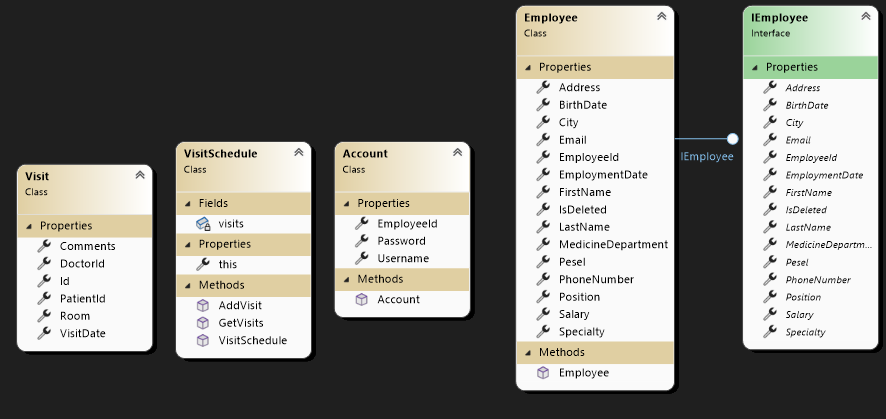
\includegraphics[height=8cm]{images/diag_gl_kl.png}
        \caption{Diagram głównych klas}
        \label{fig:diag_gl_kl}
    \end{center}
    \end{figure}

    \begin{figure}[H]
    \centering
    \subfigure{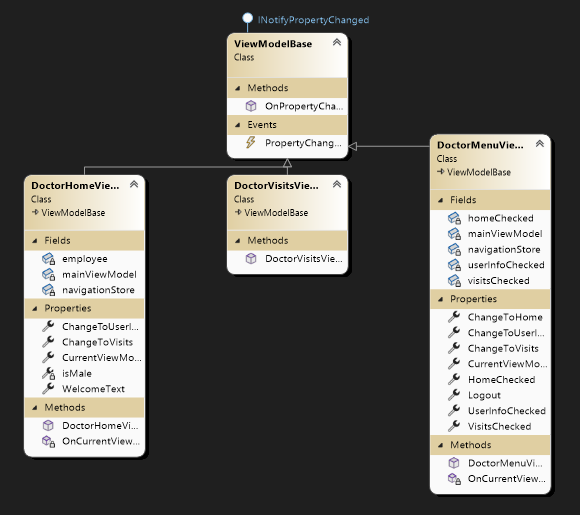
\includegraphics[width=0.4\textwidth]{images/diag_kl_nav_dok.png}} 
    \subfigure{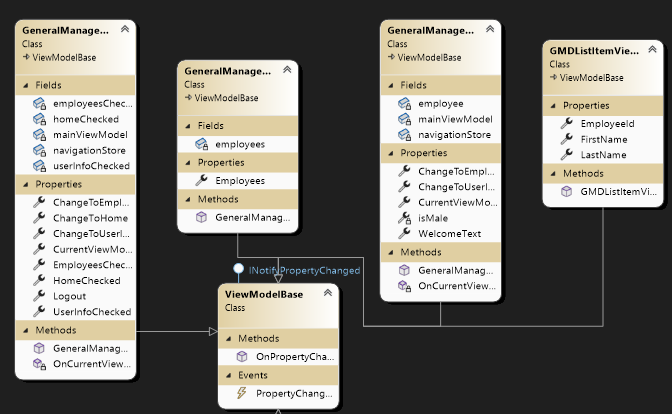
\includegraphics[width=0.5\textwidth]{images/diag_kl_nav_gen_man.png}} 
    \caption{Diagram klas nawigacyjnych dla 1)doktora 2)głównego kierownika}
 
    \label{fig:diag_kl_nav_dok_gl_kier}
    \end{figure}

    \begin{figure}[H]
    \centering
    \subfigure{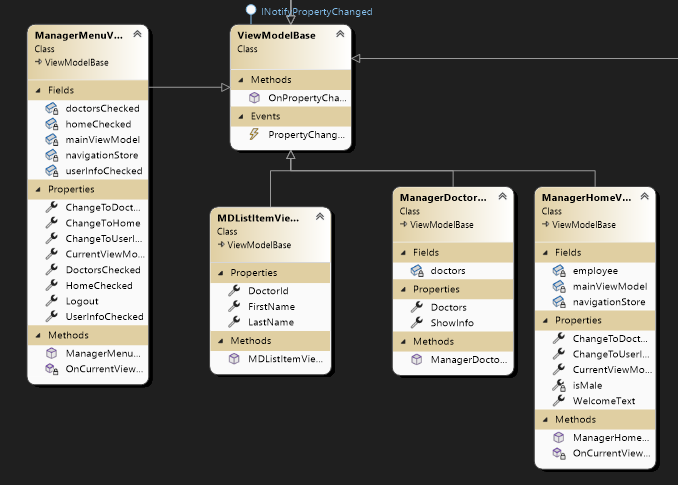
\includegraphics[width=0.4\textwidth]{images/diag_kl_nav_mang.png}} 
    \subfigure{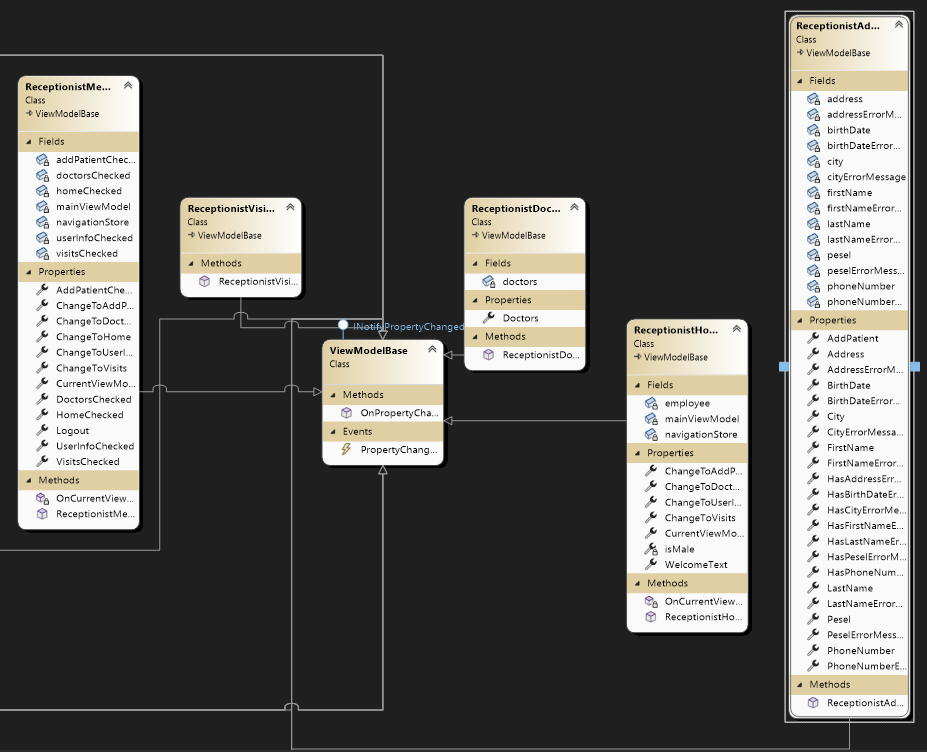
\includegraphics[width=0.4\textwidth]{images/diag_kl_nav_recep.png}} 
    \caption{Diagram klas nawigacyjnych dla 1)kierownika 2)recepcjonisty}
 
    \label{fig:diag_kl_nav_mang_recep}
    \end{figure}

    \begin{figure}[H]
    \begin{center}
	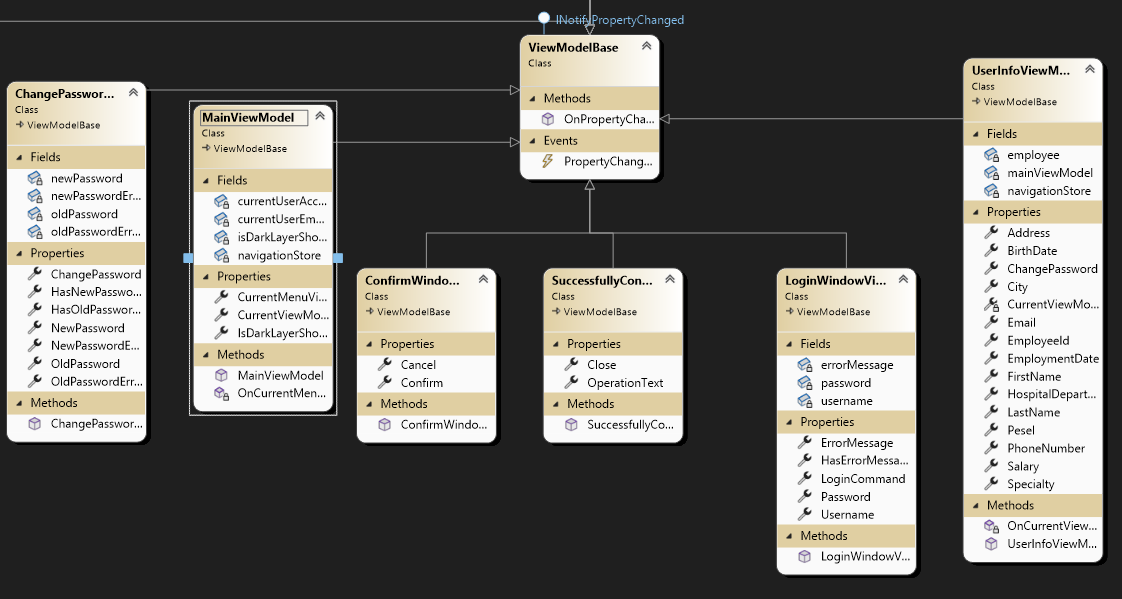
\includegraphics[height=7cm]{images/diag_kl_nav_wszt.png}
        \caption{Diagram klas nawigacyjnych dla wszystkich klientów}
        \label{fig:diag_kl_nav_recep}
    \end{center}
    \end{figure}
    
    \begin{figure}[H]
    \begin{center}
	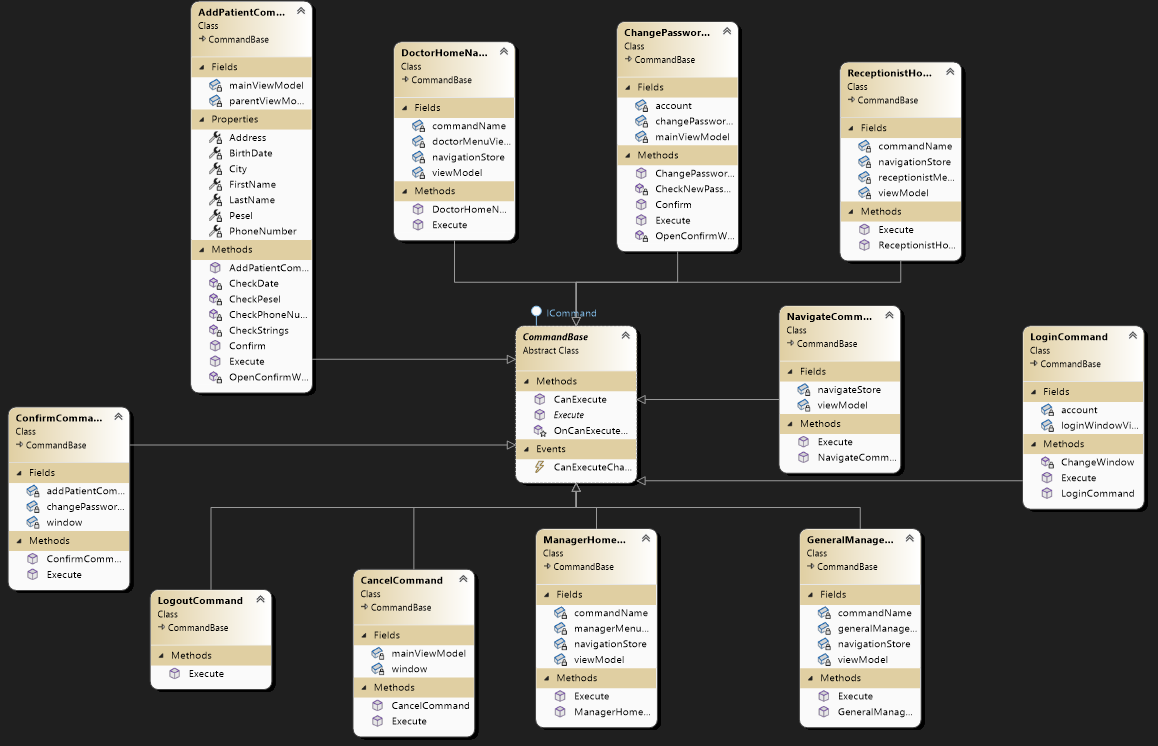
\includegraphics[height=7cm]{images/diag_kl_kom.png}
        \caption{Diagram klas komend}
        \label{fig:diag_kl_kom}
    \end{center}
    \end{figure}

    \begin{figure}[H]
    \begin{center}
	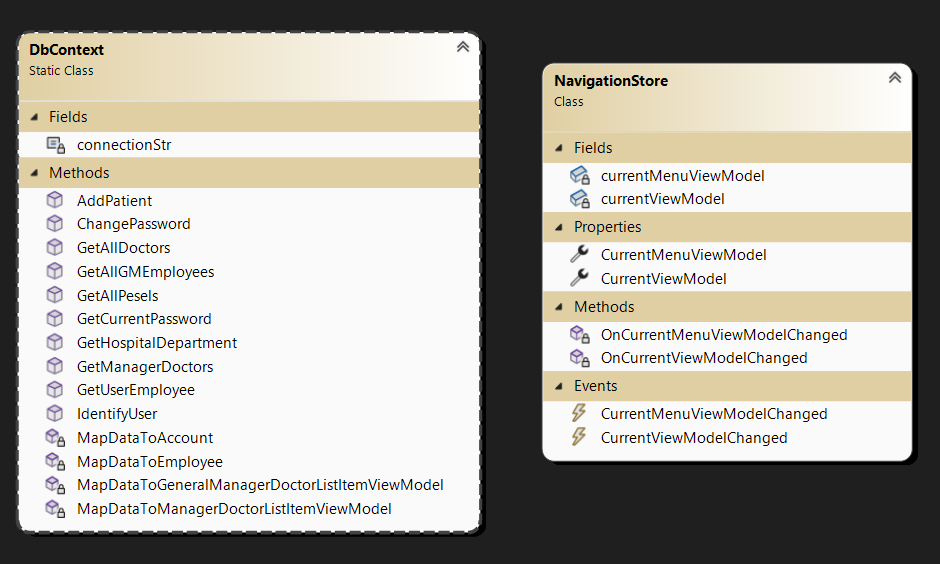
\includegraphics[height=5cm]{images/diag_kl_db_nav.png}
        \caption{Diagram klas dla bazy danych i przechowywania nawigacji}
        \label{fig:diag_kl_kom}
    \end{center}
    \end{figure}
    \subsection{\Large{Krótki opis}}
    \hspace{5mm} Projekt składa się z kilku części: Klasy główne(Models), Klasy używane do nawigacji i 
    Klasy główne używane są do przechowywania danych z bazy(np. Pracownik lub Wizyta). Klasy nawigacyjne używane są do przechowywania danych i operacji nad danymi pobranych od użytkownika w widoku(View) lub z bazy danych(np. UserInfoViewModel przechowuje informacje pobraną z bazy danych i przenosi ją do UserInfoView).
    Komendy wykorzystane są do nawigacji, przesłania danych do bazy danych lub otrzymania danych.
\end{flushleft}